\section{Exploration and organization}
\label{sec:exploration}
\rev{The rapidly growing quantity and variety of digital 3D models in large online collections have caused an emerging need to develop algorithms and techniques that effectively organize these large collections and allow users to interactively explore them.
% provide rich content that can be directly used in many applications.  For example, an architect can furnish a digital building using models from a repository.
For example, an architect might furnish a digital building by searching through databases organized according to furniture types, regions of interest and design styles.  Likewise, an industrial designer can explore shape variations among existing products when creating a new object.
%Large repositories of 3D models provide opportunities in many domains, but also necessitate developing effective tools for organizing model collections.
Most existing repositories only support text-based search, relying on user-entered tags and titles. This approach suffers from inaccurate and ambiguous tags, often entered in different languages. \rev{While it is possible to try using shape analysis to infer consistent tags as discussed in Section \ref{sec:classification}, it is difficult to convey stylistic and geometric variations using only text.} An alternative approach can be to perform shape, sketch, or image based queries. However, to formulate such search queries the user needs to have a clear mental model of the shape that should be retrieved.
Thus, some researchers focus on providing tools for \emph{exploring} shape collections. Unlike search, exploration techniques do not assume a-priori knowledge of the repository content, and help the user to understand geometric, topological, and semantic variations within the collection.}

%With the learned variations and mutual relations between different shapes,
%some works studied the organization of shape collections through grouping and relating the shapes in a systematic way.
%Combing with effective visualization, such organization can provide a global view of the entire database~\cite{Huang:2013:QOC}.

\paragraph*{Problem statement and method categorization.}
Data exploration and organization is a classical problem in data analysis and visualization~\cite{Paulovich:2011:PLP}. Given a data collection, the research focuses on \emph{grouping and relating data points, learning the data variations in the collection, and organizing the collection into a structured form},
to facilitate retrieval, browsing, summarization, and visualization of the data, based on efficient \emph{interfaces or metaphors}.

The first step to organizing model collections is to devise appropriate metrics to relate different data points. Various similarity metrics have been proposed in the past to relate entire shapes as well as local regions on shapes. In particular, previous sections of this document cover algorithms for computing global shape similarities (Section \ref{sec:classification}), part-wise correspondences (Section \ref{sec:segmentation}), and point-wise correspondences (Section \ref{sec:matching}). In this section, we will focus on techniques that take advantage of these correlations to provide different interfaces for exploring and understanding geometric variability in collections of 3D shapes.
We categorize the existing exploration approaches based on four aspects:
\begin{itemize}
\item \textbf{Metaphor:} a user interface for exploring shape variations. We will discuss five basic exploration interfaces, ones that use proxy shapes (templates), regions of interest, probability plots, query shapes, or continuous attributes.
\item \textbf{Shape comparison:} techniques used to relate different shapes. We will discuss techniques that use global shape similarities, as well as part or point correspondences.
\item \textbf{Variability:} shape variations captured by the system. Most methods we will discuss rely on geometric variability of shapes or parts. Some techniques also take advantage of topological variability; that is, variance in number of parts or how they are connected (or variance in numbers of objects and their arrangements in scenes).
\item \textbf{Organizational form:} a method to group shapes. We will discuss methods that group similar shapes to facilitate exploring intra-group similarities and inter-group variations, typically including clustering and hierarchical clustering.
\end{itemize}
Table~\ref{tab:exploration} summarizes several representative works in terms of these  aspects.
\rev{In the remaining part of this section we list several recent techniques which are grouped based on the exploration metaphor.}

\begin{table}[!t]
\centering
\begin{tabular}{l|c|c|c|c} \hline
                         Method                & Meta. & Comp. & Var.    & Org.
 \\ \hline\hline
             \cite{Ovsjanikov:2011:ECV} & temp. & simi. & geom.  & n/a
 \\ \hline   \cite{Kim:2013:lpt}         & temp. & part & both    & cluster
 \\ \hline   \cite{Averkiou:2014:spm}  	   & plot & part & both   & cluster
 \\ \hline   \cite{Kim:2012:FC}         & ROI & point & both      & n/a
 \\ \hline   \cite{Rustamov:2013:SD}  & ROI   & point & geom.     & n/a
 \\ \hline   \cite{Huang:2014:FMN}       & ROI & point & both      & cluster
 \\ \hline   \cite{Xu:2014:OHSC}         & ROI & simi. & topo.     & cluster
 \\ \hline   \cite{Fish:2014:MR}         & plot & part  & geom.     & cluster
 \\ \hline   \cite{Huang:2013:QOC}       & query & simi. & both   & hierarchy
 \\ \hline
\end{tabular}
\caption{\rev{A summary of several recent works over four aspects.
         \underline{Meta}phor: \underline{temp}lates, surface painted \underline{ROI}s,
         probability distribution \underline{plot}s, or \underline{query} shapes.
         Shape \underline{Comp}arison: shape \underline{simi}larity, \underline{part} or \underline{point} correspondence.
         \underline{Var}iability: \underline{geom}etry, \underline{topo}logy or \underline{both}.
         \underline{Org}anization Form: \underline{cluster} or \underline{hierarchy}.
         %For scene exploration, topology refers to structural graphs about scene layout~\cite{Xu:2014:OHSC}.
         }}
\label{tab:exploration}
\end{table}


\paragraph*{Template-based exploration.}
Component-wise variability in position and scale of parts reveals useful information about a model collection. Several techniques use box-like templates to show variations among models of the same class. Ovsjanikov et al.~\cite{Ovsjanikov:2011:ECV} describe a technique for learning these part-wise variations without solving the challenging problem of consistent segmentation. First, they use the segmentation of a single shape to construct the initial template. This is the only step that needs to be verified and potentially fixed by the user. The next goal is to automatically infer deformations of the template that would capture the most important geometric variations of other models in the collection.  They hypothesize that all shapes can be projected on a low-dimensional manifold based on their global shape descriptors. Finally, they reveal the manifold structure by deforming a template to fit to the sample points. Directions for interesting variations are depicted by arrows on the template and the shapes that correspond to the current template configuration are presented to the user.% \vova{perhaps we should have a figure here}.

The descriptor-based approach described above assumes that all intra-class shapes share the same parts and that there exists a low-dimensional manifold that can be captured by deforming a single template. These assumptions do not hold for large and diverse collections of 3D models.  To tackle this challenge, Kim et al.~\cite{Kim:2013:lpt} proposed an algorithm for learning several part-based templates capturing multi-modal variability in collections of shapes. They start with an initial template that includes a super-set of all parts that might occur in a dataset, and jointly learn part segmentations, point-to-point surface correspondence as well as a compact deformation model. The output is \emph{a set of templates} that groups the input models into clusters, capturing their styles and variations.

\paragraph*{ROI-based exploration.}
Not all interesting variations occur at the scale of parts: they can occur at sub-part scale, or span multiple sub-regions from multiple parts. In these cases the user may prefer to select an arbitrary region on a 3D model and look for more models sharing similar regions of interest. Such detailed and flexible queries require a finer understanding of correspondences between different shapes. Kim et al.~\cite{Kim:2012:FC} propose fuzzy point correspondences to encode the inherent ambiguity in relating diverse shapes. Fuzzy point correspondences are represented by real values specified for all pairs of points, indicating how well the points correspond.  They leverage transitivity in correspondence relationships to compute this representation from a sparse set of pairwise point correspondences.  The interface proposed by Kim et al. allows users to paint regions of interest directly on a surface and then retrieve similar regions among other shapes, or even show geometric variations found in the selected region (see Figure~\ref{fig:kim_sig12_fc}).
\begin{figure}[t]
\centering
    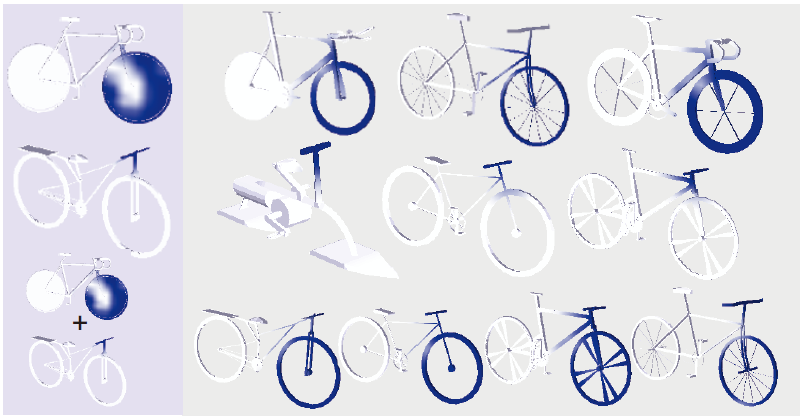
\includegraphics[width=1.0\columnwidth]{fig/img/kim_sig12_fc}
    %\vspace{-0.4cm}
    \caption{Shape exploration based on fuzzy correspondence. The user paints a region of interest (ROI) on a query shape (left column), and the method
    sorts models based on their similarity within the region (right).}
    \label{fig:kim_sig12_fc}
\end{figure}



One limitation of correspondence-based techniques is that they typically do not consider the entire collection when estimating shape differences.  Rustamov et al.~\cite{Rustamov:2013:SD} focus on a fundamental intrinsic representation for shape differences.  Starting with a functional map between two shapes, that is, a map that describes a change of functional basis, they derive a shape difference operator revealing detailed information about the location, type, and magnitude of distortions induced by a map. This makes shape difference a quantifiable object that can be co-analyzed within a context of the entire collection. They show that this deeper understanding of shape differences can help in exploration. For example, one can embed shapes in a low-dimensional space based on shape differences, or use shape difference to interpolate variations by showing ``intermediate" shapes between two regions of interest.
%
To extend these technique to man-made objects, Huang et al.~\cite{Huang:2014:FMN} construct a consistent functional basis for shape collections exhibiting large geometric and topological variability. They show that the resulting consistent maps are capable of capturing discrete topological variability, such as variance in the number of bars of the back of a chair.

\paragraph*{ROI-based scene exploration.}
Recent works on organizing and exploring 3D visual data mostly focus on object collections. Exploring 3D scenes poses additional challenges since scenes typically exhibit more structural variations. Unlike man-made objects that usually contain a handful of object parts, scenes can contain anywhere from ten to hundreds of objects.  Not only this, but the objects themselves do not typically have a prescribed rigid arrangement with respect to each other. Thus, global scene similarity metrics, such as the graph kernel based one used in \cite{Fisher:2012:CSR} are limited to organizing datasets based on very high-level features, such as scene type.
%
Xu et al.~\cite{Xu:2014:OHSC} advocate that 3D scenes should be compared from the \emph{perspective} of a particular focal point which is a representative substructure of a specific scene category. Focal points are detected through contextual analysis of a collection of scenes, resulting in a clustering
of the scene collection where each cluster is characterized by its representative focal points (see Section~\ref{sec:scene}).
%
Consequently, the focal points extracted from a scene collection can be used to organize collection into an interlinked and well-connected cluster
formation, which facilitates scene exploration. Figure~\ref{fig:xu_sig14_expl} shows an illustration of such cluster-based organization
and an exploratory path transiting between two scene clusters/categories.


%\teaser{
\begin{figure}[t]
\centering
    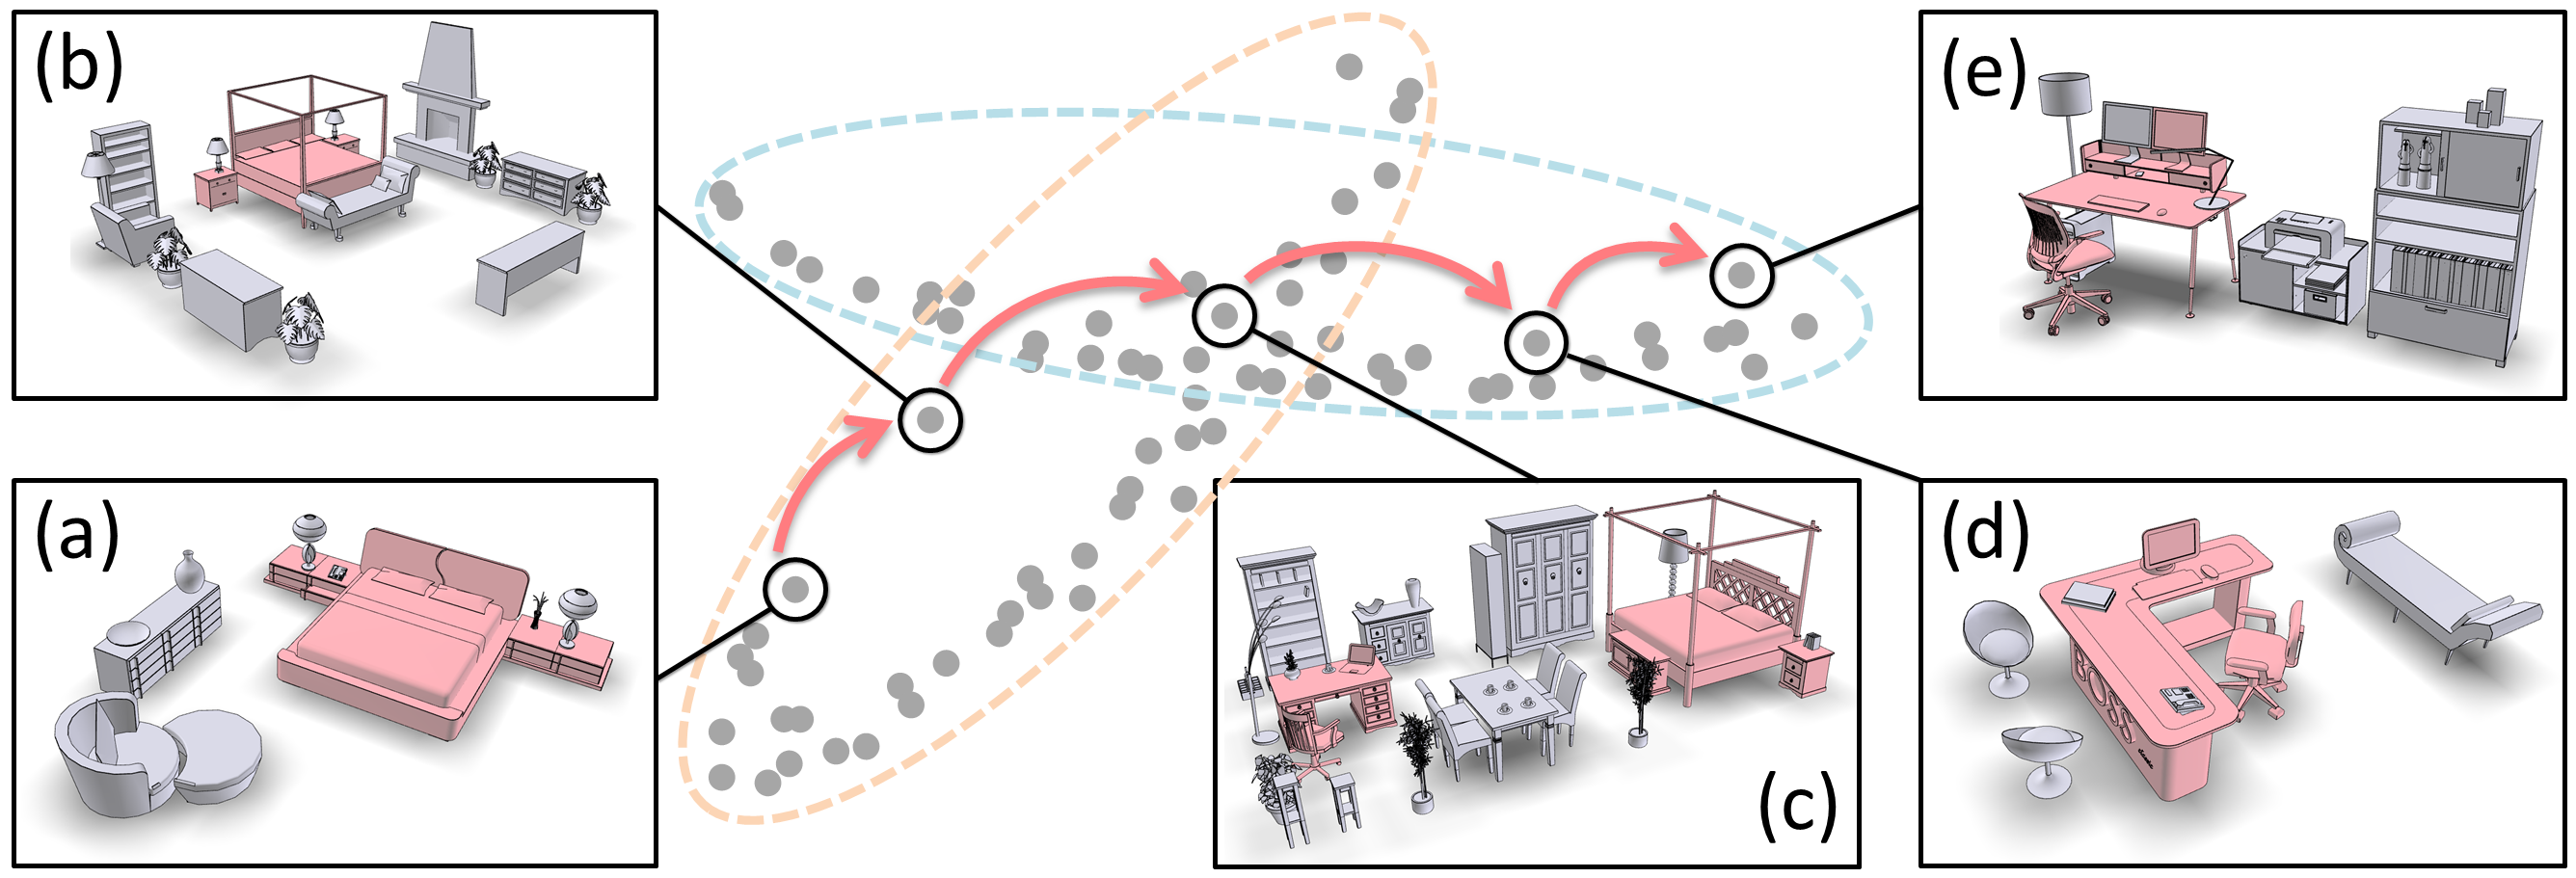
\includegraphics[width=0.99\linewidth]{fig/img/xu_sig14_expl}
%    \vspace{-0.4cm}
    \caption{
    Focal-based scene clustering produces overlapping clusters, which is due to hybrid scenes possessing multiple focal points.
    An exploratory path, from (a) to (e), through the overlap, smoothly transit between the two scene clusters,
    representing bedroom and offices, respectively.}
    \label{fig:xu_sig14_expl}
\end{figure}
%}


\paragraph*{Plot-based exploration.}
All aforementioned exploration techniques typically do not visualize the probabilistic nature of shape variations.  Fish et al.~\cite{Fish:2014:MR} study the configurations of shape parts from a probabilistic perspective, trying to indicate which shape variations are more likely to occur.  To learn the distributions of part arrangements, all shapes in the family are pre-segmented consistently.
The resulting set of probability density functions (PDFs) characterizes the variability of relations and arrangements across different parts. A peak in a PDF curve represents that particular a configuration of the related parts frequently appeared among several shapes in the family. The multiple PDFs can be used as interfaces to interactively explore the shape family from various perspectives.
Averkiou et al.~\cite{Averkiou:2014:spm} use part structure inferred by this method to produce a low-dimensional part-aware embedding of all models. The user can explore interesting variations in part arrangements simply by moving the mouse over the 2D embedding. In addition, their technique allows the synthesis of novel shapes by clicking on empty spaces in the embedded space.  Upon clicking, the system would deform parts from neighboring shapes to synthesize a novel part arrangement.

\begin{figure}[t]
\centering
    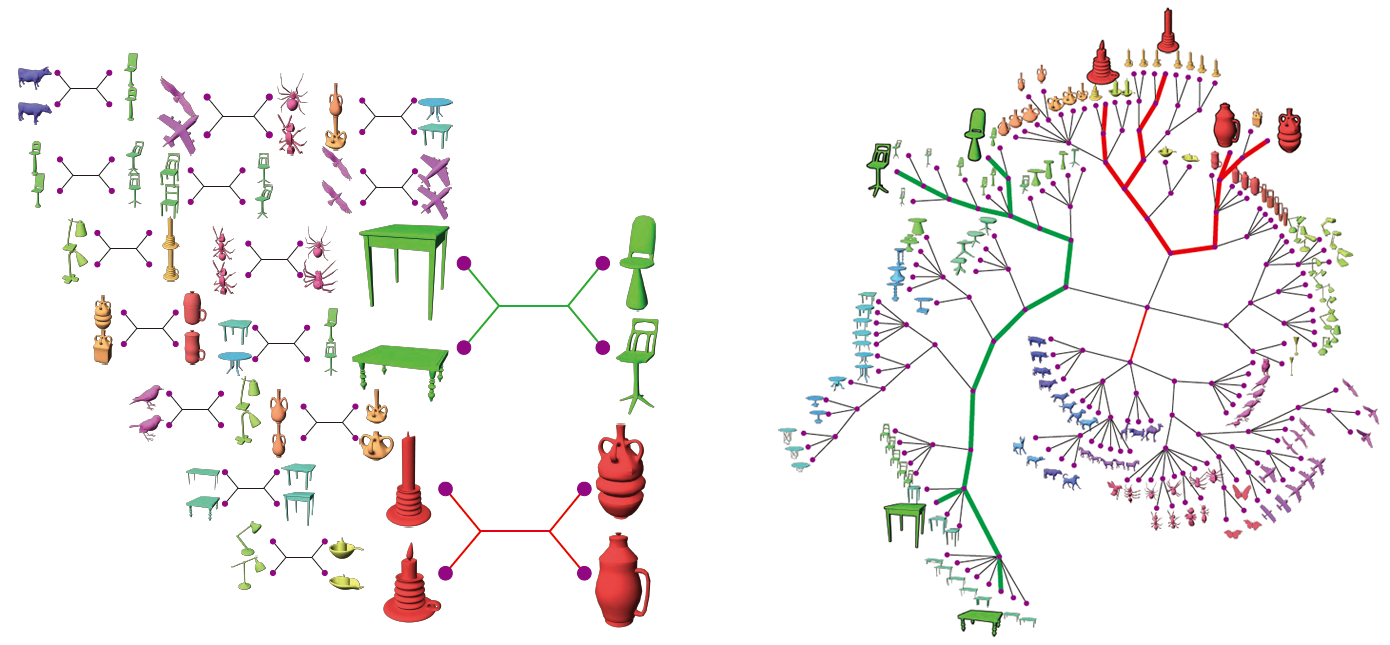
\includegraphics[width=1.0\columnwidth]{fig/img/huang_sig12_quartet}
    %\vspace{-0.4cm}
    \caption{Given a set of heterogeneous shapes, a reliable qualitative similarity is derived from quartets composed of two pairs of objects (left).
    Aggregating such qualitative information from many quartets computed across the whole set leads to a categorization tree as a hierarchical
    organization of the input shape collection (right).}
    \label{fig:huang_sig12_quartet}
\end{figure}



\paragraph*{Query-based exploration.}
For a heterogeneous shape collection encompassing diverse object classes, it is typically not possible to characterize part-structure and correspondences between all pairs of shapes. Even global shape similarity is not a very reliable feature in this setting, which makes organizing and exploring heterogeneous collections especially difficult.
To address this challenge, Huang et al.~\cite{Huang:2013:QOC} introduce qualitative analysis techniques from the field of bioinformatics. Instead of relying on quantitative distances, which may be ill-applied between dissimilar shapes, the method considers a more reliable \emph{qualitative similarity} derived from \emph{quartets} composed of two pairs of objects. The shapes that are paired in the quartet are close to each other and far from the shapes in the other pair, where distances are estimated from multiple shape descriptors.  They aggregate this topological information from many quartets computed across the entire shape collection, and construct a hierarchical \emph{categorization tree} (see Figure~\ref{fig:huang_sig12_quartet}). Analogous to the phylogenetic trees of species, this categorization tree of a shape collection provides an overview of the shapes as well as their mutual distance and hierarchical relations. Based on such an organization, they also define the degree of separation chart for every shape in the collection and apply it for interactive shape exploration.

\paragraph*{Attribute-based exploration.}
Yet another approach seeks to allow users to interactively explore shapes with continuously valued semantic attributes.  Blanz and Vetter \cite{Blanz:1999:MMS} provide an interface to explore faces based on continuous facial attributes, such as ``smile'' or ``frown'', \rev{built upon the face parametric model (Section \ref{sec:recon}}). Similarly, Allen et al.~\cite{Allen:2003:SHB} allow users to explore the range of human bodies with features such as height, weight, and age. Chaudhuri et al.'s~\cite{Chaudhuri:2013:ACC} interface enables exploration of shape parts according to learned strengths of semantic attributes (Figure \ref{fig:attribit}). 